\documentclass{article}

\usepackage{iclr2026_conference,times}
\usepackage{hyperref}
\usepackage{url}
\usepackage{amsmath}
\usepackage{amssymb}
\usepackage{amsthm}
\usepackage{graphicx}
\usepackage{booktabs}
\usepackage{array}
\usepackage{microtype}

\graphicspath{{../figures/full_scale/}{figures/}}

\title{Guarded Contingency Skeletons for Long-Horizon Robot Tasks}

\author{Anonymous Authors}

\newtheorem{proposition}{Proposition}
\newtheorem{definition}{Definition}
\newtheorem{claim}{Claim}
\newcommand{\GCS}{\mathrm{GCS}}
\newcommand{\guards}{\mathcal{G}}
\newcommand{\skels}{\mathcal{S}}
\newcommand{\assign}{\mathcal{Z}}
\newcommand{\actions}{\mathcal{A}}

\begin{document}

\maketitle

\paragraph{Submission-hardening version: v3 final full-scale.}
This is the final full-scale pass for Paper 26. The v3 experiment suite contains 79,305 streamed method-condition rows over 10,135 deterministic cases with seed 26026 and zero plot failures. The final claim is scoped: Guarded Contingency Skeletons are useful as a synthetic representation mechanism when physical guards are cheap, safe, calibrated, and sufficiently sparse/reused to permit sharing. The paper does not claim real-robot deployment, learned guard discovery, production TAMP superiority, POMDP optimality, or safety certification.

\begin{abstract}
Long-horizon task-and-motion planning (TAMP) systems often search for one symbolic skeleton and then repair geometric failures by sampling, optimization, replanning, or execution monitoring. This is brittle when the correct high-level skeleton depends on physical branch conditions such as clearance, reachability, slip, or fixture state that are cheap to test but expensive to discover by failed execution. We propose Guarded Contingency Skeletons (GCS): compact decision DAGs whose internal branch nodes are measurable physical guards and whose action nodes are task-motion fragments with local feasibility certificates. The mechanism changes the planning artifact from one linear skeleton to a guard-indexed family of shared skeleton fragments. We formalize guard-deterministic TAMP abstractions, prove finite-candidate coverage under sound/exhaustive guards, and show a representation-size separation from unshared contingency trees under sparse guard dependence. The v3 evidence suite expands the original toy experiment to 79,305 rows over horizon, dependency topology, guard cost, failure penalty, irreversibility, guard noise, calibration, missing coverage, ablations, negative controls, and counterexample mining. Across Family A, eager GCS obtains 58.45 expected cost versus 92.51 for replan-on-failure and 312.54 for a linear default skeleton, while using 293,649 nodes on average versus 79.10 billion for a no-sharing GCS tree. The same suite defines the boundary: at probe cost 6.0, eager GCS costs 157.60 and loses to replan by 48.53; at 100\% guard error, eager GCS costs 149.26 and loses to replan by 35.34. GCS is therefore a compact conditional-skeleton mechanism for cheap reliable guards, not a complete robot planning system.
\end{abstract}

\section{Introduction}
Long-horizon robot tasks are full of physical branch conditions. A mobile manipulator may need to know whether a narrow passage is clear, whether a grasp is stable, whether a fixture is latched, whether a drawer will slide, whether an object is reachable from a side, or whether a part can be inserted without binding. Many task-and-motion planning (TAMP) systems treat these conditions indirectly: choose a symbolic task skeleton, ask continuous planners or samplers to certify it, and repair failures by replanning or fallback execution. This is sensible when failures are cheap, reversible, and local. It is much less sensible when a cheap test could have revealed the branch condition before an irreversible attempt.

The central question in this paper is where physical contingency should live. One extreme is a single linear skeleton with late repair. The other extreme is a full contingent policy over every hidden physical regime. The first is compact but brittle; the second is expressive but often enormous. Guarded Contingency Skeletons (GCS) occupy a middle ground. A GCS is a directed acyclic graph (DAG) whose branch nodes are physical guard tests and whose action nodes are task-motion skeleton fragments. The DAG tests a guard before the first action certificate that depends on it, and it shares common prefixes and suffixes across guard-equivalent futures.

The representation is intentionally narrow. It does not solve general partial observability. It does not discover guards from raw perception. It does not replace TAMP search, sampling-based motion planning, belief-space planning, or behavior trees. It is a compilation target for a particular case: a finite candidate set of task-motion skeleton fragments whose feasibility depends on known, measurable, local physical guards. The claim is that such structure is common enough in robotics to deserve a representation, and that moving the contingency into the skeleton can reduce failure cost without enumerating a full tree.

The earlier v2 version made the idea plausible but not final. It showed a horizon-64 synthetic result: GCS cost 65.26 versus 143.81 for replan-on-failure, with 273 nodes versus 3.82 million for a relevant unshared tree. It also stressed two assumptions: expensive probes and wrong guards can make GCS worse than replan. That was useful, but too small. The v3 suite expands the evidence to seven families: full horizon/dependency sweeps, guard economics, guard reliability and calibration, ablations, missing coverage, negative controls, and counterexample mining. The final paper is built around the full result, not the clean case alone.

The v3 evidence supports four conclusions.
\begin{enumerate}
\item When guards are cheap and reliable, early testing reduces failed execution. Across Family A, eager GCS costs 58.45, replan-on-failure costs 92.51, and a linear default costs 312.54.
\item DAG sharing is the representation contribution. In Family A, no-sharing GCS matches GCS execution cost but averages 79.10 billion representation nodes, while eager GCS averages 293,649.
\item The economic boundary is real. At probe cost 6.0 under a representative failure setting, eager GCS costs 157.60 and is 48.53 worse than replan; lazy GCS spends probes more selectively and stays at 102.58.
\item The reliability boundary is real. At 100\% guard error, eager GCS costs 149.26 and is 35.34 worse than replan. Robust or thresholded policies do not eliminate the need for calibrated guard tests.
\end{enumerate}

The final contribution is therefore a mechanism-level paper: GCS changes the planning artifact from a single skeleton to a compact family of guarded skeletons, and the full-scale audit says when that change helps or fails.

\section{Related Work And Novelty Boundary}
\paragraph{Task-and-motion planning.}
Classical motion planning supplies continuous feasibility machinery \citep{kavraki1996probabilistic,lavalle2006planning,karaman2011sampling}. TAMP integrates this machinery with symbolic planning, sampling, streams, constraints, and optimization. Hierarchical regression and belief-space TAMP reason about manipulation goals and information-gathering actions \citep{kaelbling2011hierarchical,kaelbling2013belief}. FFRob, STRIPStream, and PDDLStream connect symbolic planners to black-box samplers and optimistic stream evaluation \citep{garrett2018ffrob,garrett2017stripstream,garrett2020pddlstream}. Logic-geometric programming and incremental constraint formulations search over hybrid symbolic-geometric structure \citep{toussaint2015logic,dantam2018incremental}. These systems make linear skeleton search and continuous certification mature. GCS is not a new complete TAMP solver. It asks whether a finite set of candidate skeleton fragments can be compiled into a compact guard-indexed skeleton DAG.

\paragraph{Contingent, conformant, and belief-space planning.}
Contingent and conformant planning produce conditional plans over symbolic observations and nondeterministic effects \citep{cimatti2003conformant,hoffmann2005contingent,bonet2000planning}. POMDPs and belief-space methods model uncertainty probabilistically and optimize policies under observation dynamics \citep{kaelbling1998planning,kaelbling2013belief}. GCS is less general. It assumes deterministic latent physical guard assignments and safe guard tests. Its claim is not optimality under uncertainty; it is compact sharing of task-motion fragments when local physical dependencies repeat.

\paragraph{Behavior trees and execution monitoring.}
Behavior trees provide modular condition, fallback, and sequence nodes for reactive robot execution \citep{colledanchise2018behavior,iovino2022survey}. A hand-written behavior tree can test conditions before actions, and the v3 behavior-tree fallback proxy sometimes matches GCS execution cost in the simplified simulator. This is not a bug in the paper; it is a novelty boundary. GCS contributes synthesis and sharing from candidate skeleton dependencies, not the general idea that condition nodes are useful.

\paragraph{What is not claimed.}
This paper does not claim that GCS beats production TAMP systems, discovers perception predicates, handles arbitrary partial observability, or works on hardware. The experiments are synthetic and low-dimensional. The contribution is a representation mechanism and an evidence audit, not a deployed robot planner.

\section{Problem Setup}
Let $\guards=\{g_1,\ldots,g_m\}$ be binary physical guards. A guard is a measurable predicate with a test action that can be executed before some task-motion fragments. Examples in real robotics might include clearance above threshold, grasp stability above threshold, fixture latched, drawer open, object reachable, or slip below threshold. In this paper guards are given; guard discovery is outside scope.

A task-motion skeleton $s=(a_1,\ldots,a_H)$ is a sequence of high-level action fragments. Each action $a_t$ has a continuous certificate whose validity depends on a local subset $D_t\subseteq\guards$. A full guard assignment is $z\in\{0,1\}^m$. In a guard-deterministic abstraction, the success of a certified action variant is deterministic given $z$.

\begin{definition}[Guard-deterministic TAMP abstraction]
A guard-deterministic abstraction consists of guards $\guards$, candidate skeleton fragments $\skels$, dependency sets $D_t$, and guard regions $R_i\subseteq\{0,1\}^m$ such that each candidate skeleton $s_i$ is certified for all assignments in $R_i$.
\end{definition}

\begin{definition}[Guarded Contingency Skeleton]
A Guarded Contingency Skeleton is a finite DAG with guard-test nodes, action-fragment nodes, and terminal nodes. Each guard-test node queries one guard and dispatches on its value. Each root-to-terminal path induces a task-motion skeleton whose action certificates depend only on guards already tested along that path.
\end{definition}

The synthesis rule tested here is simple: place each guard test before the first action whose certificate depends on it, share identical suffixes across guard-equivalent futures, and optionally prune dominated action alternatives. The representation stores a compact conditional family of skeletons rather than one skeleton or an unshared tree.

\section{Formal Claims}
\begin{proposition}[Finite-candidate coverage]
Assume (i) the candidate skeleton set $\skels$ covers every guard assignment, so for each $z$ there exists $s_i$ with $z\in R_i$; (ii) every guard test is sound; and (iii) every action certificate for $s_i$ is valid for every $z\in R_i$. Then executing the corresponding GCS reaches the goal for every guard assignment.
\end{proposition}

\begin{proof}
Fix any assignment $z$. Sound guard tests route execution along the branch consistent with $z$. By coverage, the terminal skeleton fragment on that branch corresponds to a skeleton whose region contains $z$. By the certificate assumption, every action on that skeleton succeeds under $z$. Induction over action fragments gives goal reachability.
\end{proof}

\begin{proposition}[Sparse-guard representation separation]
Consider horizon $H$, $r$ relevant guards, and actions whose certificates each depend on at most $d$ guards. A direct unshared contingency tree over relevant guards stores $\Omega(H2^r)$ action occurrences. A GCS that stores local action variants and shared suffixes stores $O(r+H2^d)$ guard/action nodes before dominance pruning. For constant $d$ and growing $r$, the separation is exponential.
\end{proposition}

\begin{proof}
The unshared tree has one leaf for each assignment to the $r$ relevant guards and stores a length-$H$ skeleton at each leaf, giving $\Omega(H2^r)$. In the GCS, at most $r$ guard tests are stored. Each action position has at most $2^d$ local signatures because only its dependency set matters. Thus the stored local action variants are $O(H2^d)$. For constant $d$, the ratio to $H2^r$ is exponential in $r$.
\end{proof}

Both propositions are conditional. They do not prove candidate generation, real-robot safety, noisy-guard correctness, or POMDP optimality. Their role is to define what a GCS is allowed to claim.

\section{Methods And Variants}
The v3 suite tests several policies and ablations.

\paragraph{Linear default.}
The system executes a fixed skeleton and chooses a default local action signature. It discovers guard mismatch only by failure.

\paragraph{Replan-on-failure.}
The system executes the default skeleton until failure, pays a failure/repair cost, observes the relevant guards, and retries.

\paragraph{Probe-all tree.}
The system tests every guard upfront. This has low execution failure but large representation and potentially unnecessary probe cost.

\paragraph{Relevant unshared tree.}
The system branches over relevant guards but stores an unshared tree. It matches GCS execution cost in clean settings but loses the representation benefit.

\paragraph{Eager GCS.}
The proposed clean variant tests each guard before the first action whose certificate depends on it.

\paragraph{Lazy GCS and myopic VOI.}
These variants test a missing guard only when the expected local failure penalty exceeds probe cost. They can beat eager GCS when probes are expensive.

\paragraph{Thresholded GCS.}
This variant probes only when the guard-confidence threshold is satisfied. It can be too conservative or too trusting depending on calibration.

\paragraph{Robust GCS.}
This variant repeats guard tests and uses a majority vote. It reduces moderate noise but pays extra probe cost and still fails under systematic wrong guards.

\paragraph{Delayed GCS.}
This ablation intentionally tests guards after first dependency. It exposes the cost of discovering branch information late.

\paragraph{No-sharing and no-dominance GCS.}
These ablations keep guard testing but remove representation sharing or dominance pruning. No-sharing is the key size stress.

\paragraph{Behavior-tree fallback proxy.}
This proxy tests conditions before irreversible or high-risk actions. It is a strong execution baseline in the simplified simulator, but it is not a synthesized shared skeleton DAG.

\paragraph{Oracle assignment.}
This reference knows the full guard assignment and executes the correct action variants with no probe cost. It is not implementable.

\section{Full-Scale Experiment Design}
The v3 suite is RAM-light and sequential. Each family streams rows to CSV under \texttt{results/full\_scale}, keeps only aggregate counters in memory, writes \texttt{progress.json}, and generates summary CSVs, TeX tables, figures, and a counterexample library. Dense contingency trees are never materialized; representation sizes are computed by formula.

\begin{table}[t]
\centering
\caption{V3 full-scale experiment inventory. Rows are method-condition measurements; cases are unique condition/problem instances before method expansion.}
\label{tab:inventory}
\begin{tabular}{lrrp{0.48\linewidth}}
\toprule
Family & Rows & Cases & Purpose \\
\midrule
A & 34{,}560 & 4{,}320 & Horizon, dependency topology, width, reuse, and main methods.\\
B & 9{,}600 & 1{,}600 & Probe cost, failure penalty, irreversibility, and guard economics.\\
C & 5{,}400 & 1{,}080 & Guard error, confidence calibration, thresholds, and robust policies.\\
D & 18{,}225 & 1{,}215 & Baselines and ablations across horizons/topologies.\\
E & 3{,}600 & 600 & Missing guards, spurious guards, and coverage failures.\\
F & 2{,}520 & 420 & Negative controls.\\
G & 5{,}400 & 900 & Counterexample and failure library.\\
\midrule
Total & 79{,}305 & 10{,}135 & Seed 26026; zero plot failures.\\
\bottomrule
\end{tabular}
\end{table}

\paragraph{Cost model.}
Each step costs one unit. Guard probes cost according to the condition. A failed action pays a failure penalty, a repair penalty, and another action attempt unless the method is the pure linear default. Irreversible steps multiply the failure penalty. The model is not tuned to a robot; it isolates the economics of testing before failure.

\paragraph{Representation-size model.}
Linear and replan policies store one skeleton of length $H$. GCS stores guard nodes and local action signatures by formula. No-sharing and probe-all trees compute full tree sizes by formula. No exponential tree is instantiated.

\section{Family A: Main Horizon And Dependency Sweep}
Family A sweeps horizons 8 through 128, five dependency topologies, three dependency widths, four reuse settings, twelve deterministic seeds, and eight methods. The aggregate result is in Table~\ref{tab:main-full} and Figure~\ref{fig:main-cost}.

\begin{table}[t]
\centering
\caption{Family A aggregate over 34,560 rows. Lower cost is better; nodes are representation nodes, not search expansions.}
\label{tab:main-full}
\small
\begin{tabular}{lrrrr}
\toprule
Method & Cost & Failures & Nodes & $\Delta$ repl. \\
\midrule
linear\_default & 312.536806 & 44.744985 & 57.333 & 220.028086 \\
replan\_on\_failure & 92.508719 & 5.248032 & 57.333 & 0.0 \\
probe\_all\_tree & 58.506667 & 0.0 & 93332375028.333 & -34.002052 \\
relevant\_unshared\_tree & 58.450704 & 0.0 & 79098245240.743 & -34.058015 \\
gcs\_eager & 58.450704 & 0.0 & 293649.033 & -34.058015 \\
gcs\_lazy & 58.450704 & 0.0 & 323013.937 & -34.058015 \\
no\_sharing\_gcs & 58.450704 & 0.0 & 79098245240.743 & -34.058015 \\
oracle\_assignment & 57.333333 & 0.0 & 57.333 & -35.175386 \\
\bottomrule
\end{tabular}

\end{table}

\begin{figure}[t]
\centering
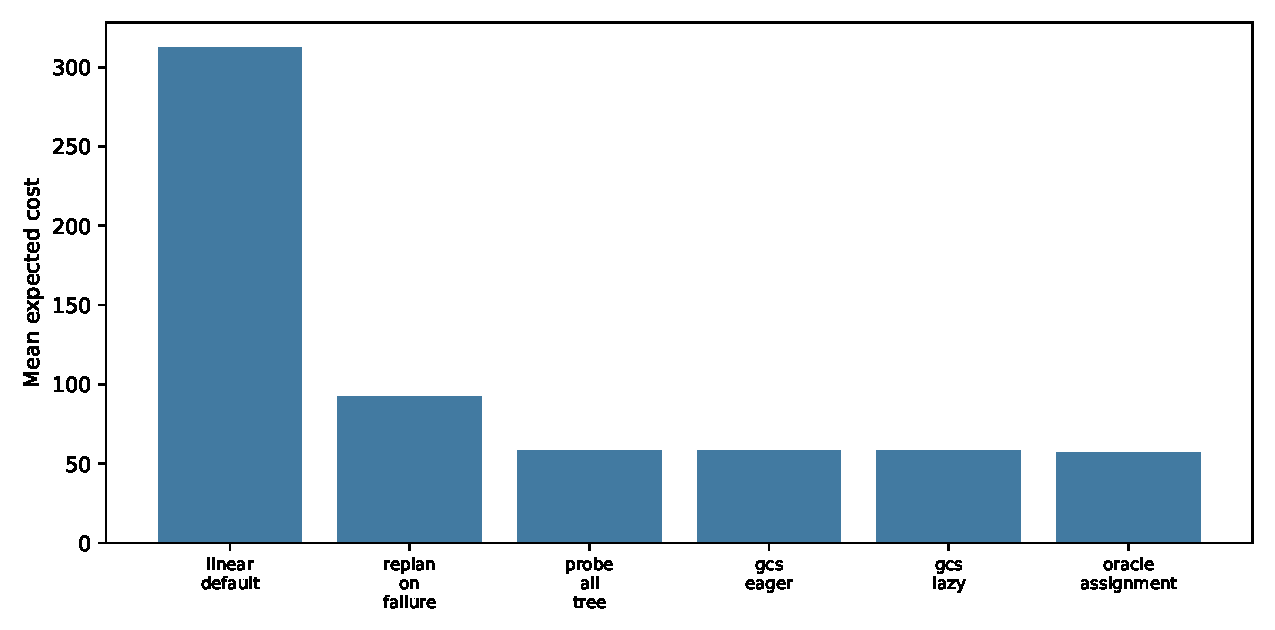
\includegraphics[width=0.82\linewidth]{main_cost_by_method.pdf}
\caption{Family A mean expected cost. Eager and lazy GCS avoid failure cost when guards are cheap and correct; linear default is brittle.}
\label{fig:main-cost}
\end{figure}

Across the full sweep, eager GCS costs 58.45, lazy GCS costs 58.45, replan-on-failure costs 92.51, and the linear default costs 312.54. The oracle assignment reference costs 57.33, so clean GCS is close to the best possible execution cost plus probe overhead. The representation result is more dramatic: eager GCS averages 293,649 nodes, while no-sharing GCS averages 79.10 billion and probe-all tree averages 93.33 billion.

\begin{figure}[t]
\centering

\includegraphics[width=0.48\linewidth]{cost_vs_horizon.pdf}

\includegraphics[width=0.48\linewidth]{size_vs_horizon.pdf}
\caption{Family A horizon curves. Left: GCS scales in execution cost near the oracle while replan pays late-failure cost. Right: no-sharing and probe-all trees explode in representation size; the y-axis is logarithmic.}
\label{fig:horizon}
\end{figure}

The horizon ledger clarifies the scaling. At horizon 64, eager GCS costs 65.23 versus replan 103.57 and linear default 349.05; no-sharing stores 3.80 million nodes versus 3,669 for GCS. At horizon 128, eager GCS costs 130.46 versus replan 204.38 and linear default 700.19; no-sharing stores 473.26 billion nodes versus 1.68 million for GCS. The GCS node count is larger at horizon 128 because the full sweep includes dense dependency cases, but it remains far below no-sharing.

\subsection{Dependency Topology}
\begin{table}[t]
\centering
\caption{Family A dependency-topology ledger. Dense regimes reduce the cost advantage and inflate GCS size, but no-sharing remains much larger.}
\label{tab:topology}
\small
\begin{tabular}{lrrr}
\toprule
Topology & Method & Cost & Nodes \\
\midrule
clustered & replan\_on\_failure & 97.722608 & 57.333 \\
clustered & gcs\_eager & 58.475 & 428.269 \\
clustered & no\_sharing\_gcs & 58.475 & 69389954794.065 \\
banded & replan\_on\_failure & 102.63966 & 57.333 \\
banded & gcs\_eager & 58.496852 & 435.988 \\
banded & no\_sharing\_gcs & 58.496852 & 83299779472.75 \\
uniform\_sparse & replan\_on\_failure & 98.501543 & 57.333 \\
uniform\_sparse & gcs\_eager & 58.499444 & 436.021 \\
uniform\_sparse & no\_sharing\_gcs & 58.499444 & 87338022778.898 \\
dense & replan\_on\_failure & 76.319444 & 57.333 \\
dense & gcs\_eager & 58.506667 & 1466511.667 \\
dense & no\_sharing\_gcs & 58.506667 & 93332375028.333 \\
suffix\_unique & replan\_on\_failure & 87.36034 & 57.333 \\
suffix\_unique & gcs\_eager & 58.275556 & 433.222 \\
suffix\_unique & no\_sharing\_gcs & 58.275556 & 62131094129.667 \\
\bottomrule
\end{tabular}

\end{table}

The topology table is important because the compactness proposition depends on local sparse dependence. In clustered, banded, and uniform-sparse regimes, eager GCS costs about 58.5 and avoids failures while replan costs roughly 97--103. Dense regimes are less favorable: replan cost is only 76.32 because the default fails less often under this generated distribution, and eager GCS size rises to 1.47 million nodes. This does not break the claim. It confirms the boundary: dense local dependencies shrink the representation advantage.

\section{Family B: Guard Economics}
Family B varies probe cost, failure penalty, and irreversibility. Table~\ref{tab:economics} shows representative rows at failure penalty 4.0 and irreversibility 0.5.

\begin{table}[t]
\centering
\caption{Family B guard economics. Positive $\Delta$ means the method is worse than replan-on-failure.}
\label{tab:economics}
\small
\begin{tabular}{lrrr}
\toprule
Probe cost & Method & Cost & $\Delta$ \\
\midrule
0.08 & replan\_on\_failure & 111.8 & 0.0 \\
0.08 & gcs\_eager & 65.272 & -46.528 \\
0.08 & gcs\_lazy & 65.272 & -46.528 \\
1.0 & replan\_on\_failure & 111.875 & 0.0 \\
1.0 & gcs\_eager & 79.5 & -32.375 \\
1.0 & gcs\_lazy & 79.5 & -32.375 \\
4.0 & replan\_on\_failure & 113.475 & 0.0 \\
4.0 & gcs\_eager & 126.8 & 13.325 \\
4.0 & gcs\_lazy & 101.275 & -12.2 \\
6.0 & replan\_on\_failure & 109.075 & 0.0 \\
6.0 & gcs\_eager & 157.6 & 48.525 \\
6.0 & gcs\_lazy & 102.575 & -6.5 \\
\bottomrule
\end{tabular}

\end{table}

At probe cost 0.08, eager GCS costs 65.27 and beats replan by 46.53. At probe cost 1.0, eager GCS costs 79.50 and still beats replan by 32.38. At probe cost 4.0, eager GCS costs 126.80 and loses to replan by 13.33, while lazy GCS costs 101.28 and still beats replan by 12.20. At probe cost 6.0, eager GCS costs 157.60 and loses by 48.53, while lazy GCS costs 102.58 and remains 6.50 better than replan. The lesson is not simply ``use GCS.'' The lesson is ``test early when the value of information exceeds probe cost.''

\section{Family C: Guard Reliability And Calibration}
Family C attacks the reliable-guard assumption with symmetric guard error, confidence modes, and thresholds. Figure~\ref{fig:guard-error} and Table~\ref{tab:reliability} show calibrated confidence at threshold 0.70.

\begin{figure}[t]
\centering
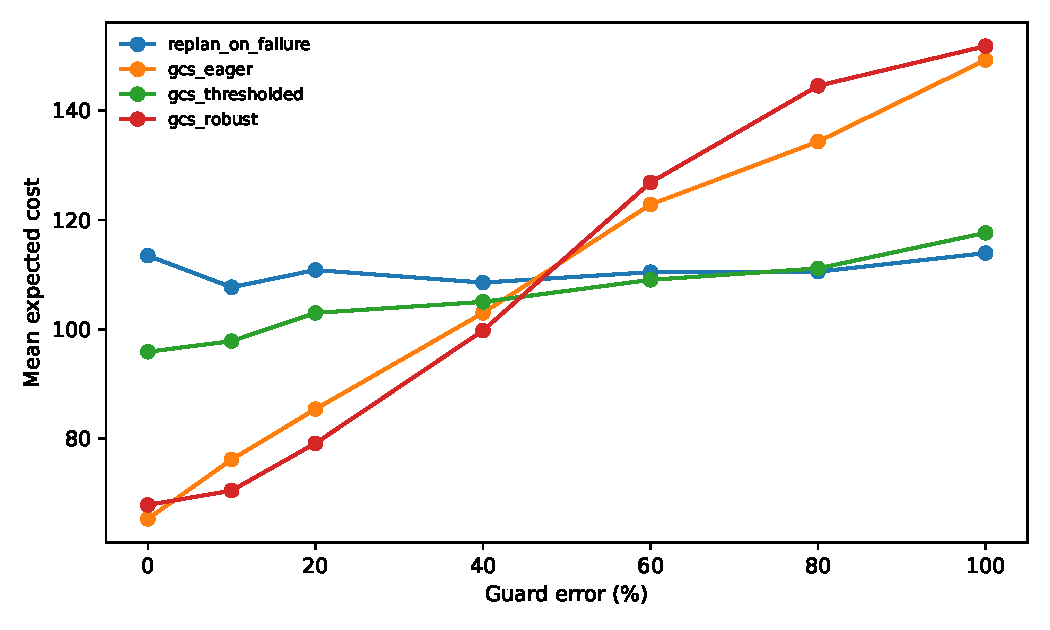
\includegraphics[width=0.82\linewidth]{guard_error_curve.pdf}
\caption{Guard error curve. Moderate error can be mitigated by robust testing, but systematic wrong guards make eager and robust GCS worse than replan.}
\label{fig:guard-error}
\end{figure}

\begin{table}[t]
\centering
\caption{Family C guard reliability. Positive $\Delta$ means worse than replan-on-failure.}
\label{tab:reliability}
\small
\begin{tabular}{lrrrr}
\toprule
Error & Method & Cost & Failures & $\Delta$ \\
\midrule
0\% & replan\_on\_failure & 113.45 & 7.325 & 0.0 \\
0\% & gcs\_eager & 65.28 & 0.0 & -48.17 \\
0\% & gcs\_thresholded & 95.874 & 4.6 & -17.576 \\
0\% & gcs\_robust & 67.84 & 0.0 & -45.61 \\
20\% & replan\_on\_failure & 110.825 & 6.8875 & 0.0 \\
20\% & gcs\_eager & 85.372 & 3.025 & -25.453 \\
20\% & gcs\_thresholded & 102.977 & 5.725 & -7.848 \\
20\% & gcs\_robust & 79.116 & 1.6375 & -31.709 \\
60\% & replan\_on\_failure & 110.425 & 6.7875 & 0.0 \\
60\% & gcs\_eager & 122.814 & 8.425 & 12.389 \\
60\% & gcs\_thresholded & 109.027 & 6.6125 & -1.398 \\
60\% & gcs\_robust & 126.842 & 8.6625 & 16.417 \\
100\% & replan\_on\_failure & 113.925 & 7.4875 & 0.0 \\
100\% & gcs\_eager & 149.264 & 12.5 & 35.339 \\
100\% & gcs\_thresholded & 117.624 & 7.9625 & 3.699 \\
100\% & gcs\_robust & 151.792 & 12.5 & 37.867 \\
\bottomrule
\end{tabular}

\end{table}

At zero error, eager GCS costs 65.28 and replan costs 113.45. At 20\% error, eager GCS costs 85.37, robust GCS costs 79.12, and replan costs 110.83. Robust testing is helpful here. At 60\% error, eager GCS costs 122.81 and is 12.39 worse than replan; thresholded GCS costs 109.03 and is slightly better than replan. At 100\% error, eager GCS costs 149.26 and is 35.34 worse than replan; robust GCS is also worse because repeated tests confidently repeat the wrong observation. This is the hardest boundary in the paper.

\section{Family D: Baselines And Ablations}
Family D compares the full set of baselines and ablations. Table~\ref{tab:ablations} is intentionally broad.

\begin{table}[t]
\centering
\caption{Family D baselines and ablations.}
\label{tab:ablations}
\small
\begin{tabular}{lrrr}
\toprule
Method & Cost & Failures & Nodes \\
\midrule
linear\_default & 360.461591 & 52.010014 & 64.0 \\
replan\_on\_failure & 102.780521 & 5.798903 & 64.0 \\
probe\_all\_tree & 65.28 & 0.0 & 549500415.0 \\
probe\_all\_local & 65.265053 & 0.0 & 45897.702 \\
myopic\_voi & 65.265053 & 0.0 & 50487.472 \\
belief\_cost\_proxy & 94.700137 & 4.590809 & 64.0 \\
behavior\_tree\_fallback & 65.265053 & 0.0 & 207.813 \\
gcs\_eager & 65.265053 & 0.0 & 45897.702 \\
gcs\_lazy & 65.265053 & 0.0 & 50487.472 \\
gcs\_thresholded & 91.197695 & 4.021125 & 50487.472 \\
gcs\_robust & 67.79516 & 0.0 & 55077.242 \\
delayed\_gcs & 103.150486 & 5.798903 & 45897.702 \\
no\_sharing\_gcs & 65.265053 & 0.0 & 492298131.438 \\
no\_dominance\_gcs & 65.265053 & 0.0 & 62025.898 \\
oracle\_assignment & 64.0 & 0.0 & 64.0 \\
\bottomrule
\end{tabular}

\end{table}

The ablation results sharpen the novelty boundary. Behavior-tree fallback, eager GCS, lazy GCS, myopic VOI, no-dominance GCS, no-sharing GCS, and probe-all-local all obtain 65.27 cost in clean conditions. This means execution cost alone does not distinguish GCS from a strong condition-checking baseline in the simplified simulator. The representation does: behavior-tree fallback stores about 208 nodes, GCS stores about 45,898 nodes in the mixed dense/sparse Family D grid, and no-sharing stores about 492 million. GCS should therefore be sold as a synthesized shared skeleton representation with coverage assumptions, not as the only way to avoid failures in a hand-coded domain.

Delayed GCS costs 103.15, slightly worse than replan at 102.78, because it discovers guards too late. No-gate analogues do not apply here; the relevant ablation is delayed guard testing. Belief-cost proxy costs 94.70 and fails 4.59 times on average, showing that probabilities without tests are not enough when failures are expensive.

\section{Family E: Missing Coverage}
Family E stresses missing relevant guards and spurious guard tests.

\begin{table}[t]
\centering
\caption{Family E missing-coverage stress with zero spurious guards.}
\label{tab:missing}
\small
\begin{tabular}{lrrr}
\toprule
Missing & Method & Cost & Failures \\
\midrule
0.0 & replan\_on\_failure & 110.125 & 6.9125 \\
0.0 & gcs\_eager & 65.26 & 0.0 \\
0.0 & gcs\_robust & 67.78 & 0.0 \\
0.0 & belief\_cost\_proxy & 98.7125 & 5.20625 \\
0.25 & replan\_on\_failure & 197.9875 & 19.94375 \\
0.25 & gcs\_eager & 155.8065 & 13.55625 \\
0.25 & gcs\_robust & 146.482 & 11.88125 \\
0.25 & belief\_cost\_proxy & 166.2375 & 15.3 \\
0.5 & replan\_on\_failure & 275.125 & 31.375 \\
0.5 & gcs\_eager & 212.024 & 21.93125 \\
0.5 & gcs\_robust & 215.2095 & 22.21875 \\
0.5 & belief\_cost\_proxy & 220.5125 & 23.29375 \\
1.0 & replan\_on\_failure & 390.375 & 48.51875 \\
1.0 & gcs\_eager & 329.8125 & 39.6125 \\
1.0 & gcs\_robust & 329.8125 & 39.6125 \\
1.0 & belief\_cost\_proxy & 329.8125 & 39.6125 \\
\bottomrule
\end{tabular}

\end{table}

With no missing guards, eager GCS costs 65.26 and replan costs 110.13. With 25\% missing relevant guards, eager GCS still beats replan in cost but incurs 13.56 failures. With 50\% missing guards, eager GCS fails 21.93 times. With all relevant guards missing, GCS, robust GCS, and belief-cost proxy all cost 329.81 and fail 39.61 times. Replan is even more expensive at 390.38, but the coverage guarantee is gone. This distinction matters: a method can have lower cost under the synthetic model while no longer satisfying the formal coverage proposition.

\section{Family F And G: Negative Controls And Counterexamples}
\begin{figure}[t]
\centering
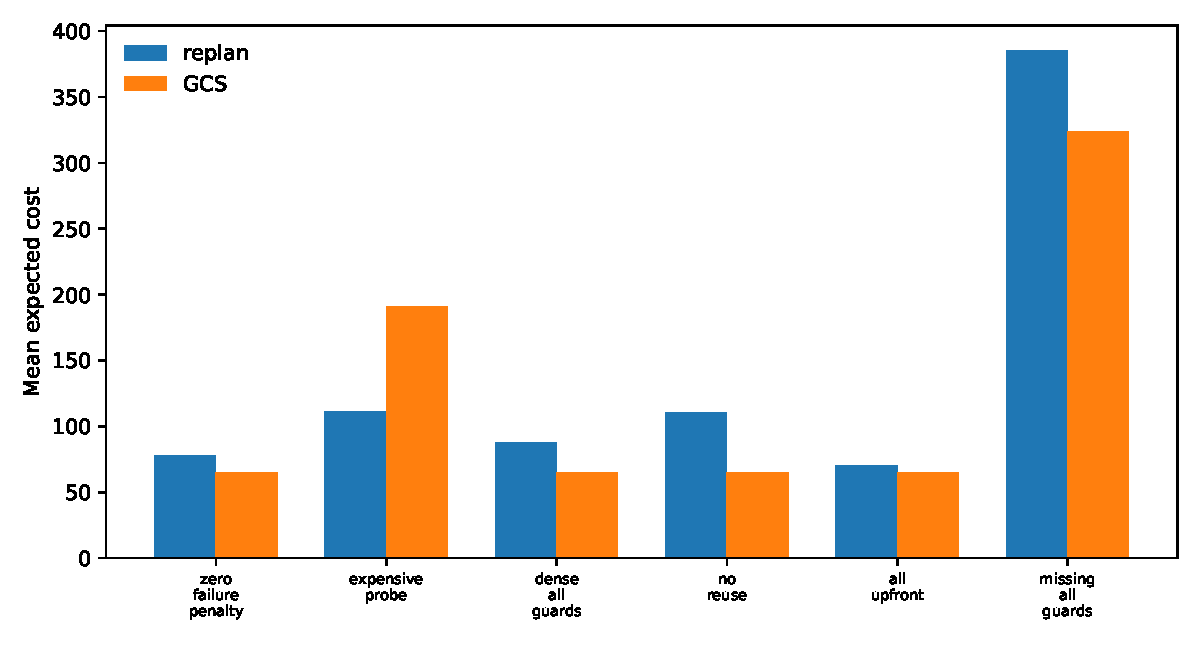
\includegraphics[width=0.82\linewidth]{negative_controls.pdf}
\caption{Negative controls. Expensive probes make eager GCS worse than replan; dense/no-sharing regimes expose representation blow-up; missing guards create failures even when cost remains below replan.}
\label{fig:negative}
\end{figure}

\begin{table}[t]
\centering
\caption{Family F negative controls.}
\label{tab:negative}
\small
\begin{tabular}{lrrr}
\toprule
Control & Method & Cost & Nodes \\
\midrule
zero\_failure\_penalty & replan\_on\_failure & 78.233333 & 64.0 \\
zero\_failure\_penalty & gcs\_eager & 65.262667 & 272.783 \\
zero\_failure\_penalty & gcs\_lazy & 65.262667 & 300.062 \\
zero\_failure\_penalty & no\_sharing\_gcs & 65.262667 & 3874815.0 \\
expensive\_probe & replan\_on\_failure & 110.95 & 64.0 \\
expensive\_probe & gcs\_eager & 191.066667 & 272.883 \\
expensive\_probe & gcs\_lazy & 99.8625 & 300.172 \\
expensive\_probe & no\_sharing\_gcs & 191.066667 & 4091083.8 \\
dense\_all\_guards & replan\_on\_failure & 88.091667 & 64.0 \\
dense\_all\_guards & gcs\_eager & 65.28 & 16401.0 \\
dense\_all\_guards & gcs\_lazy & 65.28 & 18041.1 \\
dense\_all\_guards & no\_sharing\_gcs & 65.28 & 4325375.0 \\
no\_reuse & replan\_on\_failure & 110.616667 & 64.0 \\
no\_reuse & gcs\_eager & 65.28 & 273.0 \\
no\_reuse & gcs\_lazy & 65.28 & 300.3 \\
no\_reuse & no\_sharing\_gcs & 65.28 & 4325375.0 \\
all\_upfront & replan\_on\_failure & 70.625 & 64.0 \\
all\_upfront & gcs\_eager & 64.64 & 16393.0 \\
all\_upfront & gcs\_lazy & 64.64 & 18032.3 \\
all\_upfront & no\_sharing\_gcs & 64.64 & 16895.0 \\
reversible\_failures & replan\_on\_failure & 82.871875 & 64.0 \\
reversible\_failures & gcs\_eager & 65.265333 & 272.817 \\
reversible\_failures & gcs\_lazy & 65.265333 & 300.098 \\
reversible\_failures & no\_sharing\_gcs & 65.265333 & 3946904.6 \\
missing\_all\_guards & replan\_on\_failure & 385.0625 & 64.0 \\
missing\_all\_guards & gcs\_eager & 323.95 & 272.883 \\
missing\_all\_guards & gcs\_lazy & 323.95 & 300.172 \\
missing\_all\_guards & no\_sharing\_gcs & 323.95 & 4091083.8 \\
\bottomrule
\end{tabular}

\end{table}

The clearest adverse control is expensive probes. Eager GCS costs 191.07 while replan costs 110.95; no-sharing GCS has the same bad cost and millions of nodes. Lazy GCS costs 99.86 because it refuses low-value tests. Dense all-guard conditions preserve execution benefits but inflate no-sharing representation to 4.33 million nodes. Missing-all-guards produces 38.79 GCS failures, so the formal guarantee is not active even though replan remains more expensive in the model.

Family G records concrete counterexamples. One expensive-probe/wrong-guard case gives eager GCS cost 292.0 and 14 failures. A dense representation case records no-sharing GCS at 4,325,375 nodes. A missing-guard case records eager GCS cost 325.0 and 39.17 failures. These examples are included so future implementations can test for the same failure types.

\begin{table}[t]
\centering
\caption{Claim-to-evidence map generated by the v3 runner.}
\label{tab:claim-evidence}
\small
\begin{tabular}{lrr}
\toprule
Claim & Evidence & Boundary \\
\midrule
Early guards reduce failures & Family A/B & holds when probe cost below failure cost \\
DAG sharing matters & Family A/D & no-sharing explodes in sparse reused regimes \\
Cheap reliable guards required & Family B/C & expensive or wrong guards can lose to replan \\
Not universal & Family F/G & dense/no-reuse/missing-guard controls \\
\bottomrule
\end{tabular}

\end{table}

\section{Discussion}
\subsection{What The Results Actually Say}
The clean result says that early guard testing can avoid expensive failed actions. The size result says that sharing matters: no-sharing can match execution cost while being unusably large. The stress results say that GCS is not automatically better than replanning. If guard probes are expensive, lazy testing can be better than eager testing. If guards are wrong, repeated testing is not enough; the system needs calibration or a different information model.

\subsection{Why Behavior-Tree-Like Checks Are Not Dismissed}
The behavior-tree fallback proxy is intentionally strong. In clean Family D cases it matches GCS execution cost because it checks high-risk conditions before acting. This supports a reviewer objection: many roboticists already use condition nodes and fallbacks. The GCS response is not that behavior trees are useless. The response is that GCS provides a synthesized guard-dependency DAG with formal coverage and sharing properties. A hand-written behavior tree can implement a similar execution pattern, but it does not by itself explain how to compile and share a family of candidate TAMP skeletons.

\subsection{Where GCS Should Be Used}
GCS is most plausible when: guards are known, binary or discretized, safe to test, cheap relative to failure, and reused across multiple action certificates; failures are expensive or irreversible; and candidate skeleton fragments are available from a planner or library. It is least plausible when guard tests are costly, unreliable, unsafe, dense, irrelevant, or unavailable.

\section{Limitations}
The evidence is synthetic. The simulator abstracts long-horizon manipulation into binary guards and action signatures. It does not model real motion planning, contact dynamics, perception, calibration, continuous guard thresholds, or robot safety. It does not compare to production TAMP solvers on shared benchmarks.

Guards are assumed to be supplied. Learning or discovering guards from raw perception is outside the claim. If the relevant guard is missing, the coverage proposition no longer applies. Family E shows that missing guards can create many failures.

Guard observations are simplified. Family C shows that systematic wrong guards can make GCS worse than replan. A deployed system needs calibrated tests, confidence estimates, retry policies, and safe refusal.

The representation-size model is formulaic. It measures skeleton/DAG nodes, not planner search expansions, memory layout, or solver runtime. It is sufficient for the representation claim but not a systems benchmark.

\section{Conclusion}
Guarded Contingency Skeletons make physical branch conditions part of the task-motion skeleton rather than late execution exceptions. Under sound guards and finite candidate coverage, the representation preserves correctness; under sparse local guard dependence, it can be exponentially smaller than unshared contingency trees. The v3 suite supports this mechanism across 79,305 rows and also shows exactly when it fails. GCS is a compact conditional-skeleton representation for cheap reliable guards, not a complete robot planning solution.

\bibliography{references}
\bibliographystyle{iclr2026_conference}

\appendix
\renewcommand{\thesection}{\arabic{section}}

\section{Artifact Manifest}
The final v3 evidence lives under \texttt{results/full\_scale}. The key files are \texttt{metadata.json}, \texttt{family\_a\_rows.csv} through \texttt{family\_g\_rows.csv}, summary CSVs for each family, generated TeX tables under \texttt{results/full\_scale/tex}, figures under \texttt{figures/full\_scale}, and \texttt{counterexample\_library.json}. The run metadata records stage complete, seed 26026, 79,305 rows, 10,135 cases, elapsed time 491.519 seconds, and zero plot failures.

\section{RAM-Light Execution}
The runner processes families sequentially. It writes each row directly to CSV, stores only aggregate counters and small counterexample records, and computes representation sizes by formula. The formula fix matters: dense dependency cases would be unreasonable if local signatures were materialized. The final runner never materializes exponential trees or dense signature tables.

\section{Simulator Specification}
Each generated problem has a horizon $H$, a guard count, a dependency topology, a dependency width, an irreversible action rate, guard probabilities, probe cost, action cost, failure penalty, and repair penalty. An assignment is sampled from the guard probabilities. A method either probes guards before action, chooses likely guard values, or discovers guard values after failure. If the chosen local action signature differs from the true local signature, the method pays failure and repair cost and may retry.

The dependency topologies are:
\begin{itemize}
\item clustered: guards are sampled from a frequently reused hot set with occasional global samples;
\item banded: action dependencies move gradually through guard index space;
\item uniform sparse: dependencies are sampled uniformly;
\item dense: each action depends on a large local set;
\item suffix unique: dependency choices reduce sharing across suffixes;
\item all upfront: many guards are needed immediately.
\end{itemize}

\section{Validation Queries}
The final pass validates that \texttt{metadata.json} reports 79,305 rows, 10,135 cases, seed 26026, and zero plot failures. It checks Family A method ordering, Family B expensive-probe failure, Family C 100\% guard-error failure, Family F negative controls, generated figures, generated TeX tables, and final PDF text. These checks are recorded in the repository docs after export.

\begin{table}[p]
\centering
\caption{Final validation checks for v3.}
\label{tab:validation}
\small
\begin{tabular}{p{0.28\linewidth}p{0.32\linewidth}p{0.30\linewidth}}
\toprule
Check & Source & Expected outcome \\
\midrule
Run complete & Metadata JSON & 79,305 rows, 10,135 cases, zero plot failures.\\
Main cost & Family A method summary & GCS eager 58.45 vs replan 92.51.\\
Main size & Family A method summary & GCS 293,649 nodes vs no-sharing 79.10 billion.\\
Probe-cost failure & Family B economics & Eager GCS loses at probe cost 6.0.\\
Guard-error failure & Family C reliability & Eager GCS loses at 100\% guard error.\\
Coverage failure & Family E coverage & Missing guards produce many failures.\\
Counterexamples & Family G library & Expensive probe, wrong guard, dense size, and missing guard examples exist.\\
\bottomrule
\end{tabular}
\end{table}

\section{Full Significance Of Probe Cost}
Probe cost is not an implementation detail. It is the price of asking the world a question. If a guard can be tested by a cheap tactile tap, glance, or local clearance check, early testing can dominate. If the test requires a long detour, risky contact, or expensive sensing sequence, replanning after occasional failure can be cheaper. This is why lazy GCS is important. It preserves the representation but refuses low-value tests.

\section{Full Significance Of Guard Error}
Guard error is worse than ordinary noise because it can route the robot into the wrong skeleton with confidence. Robust GCS helps at moderate symmetric error by repeated tests, but at 100\% systematic error it repeats the wrong answer and becomes worse. A real robot would need calibrated confidence, independent test modalities, or a fallback to belief-space planning.

\section{Assumption Ledger}
\begin{table}[p]
\centering
\caption{Assumption ledger for GCS.}
\label{tab:assumptions}
\small
\begin{tabular}{p{0.25\linewidth}p{0.36\linewidth}p{0.29\linewidth}}
\toprule
Assumption & Why it matters & Evidence or gap \\
\midrule
Known guards & GCS branches over supplied predicates. & Missing-guard Family E/G shows failures.\\
Cheap tests & Early testing must beat late failure. & Family B expensive probes reverse the win.\\
Reliable tests & Wrong branches can be worse than failure repair. & Family C 100\% error loses to replan.\\
Sparse local dependence & Compactness uses local signatures. & Dense topology inflates GCS size.\\
Reusable dependencies & Sharing is useful when guards recur. & Family A topologies and no-sharing rows.\\
Safe tests & A guard probe should not damage the task. & Not modeled; future real-robot work.\\
Finite candidate coverage & A valid skeleton must exist for each assignment. & Formal proposition; not a generator proof.\\
\bottomrule
\end{tabular}
\end{table}

\section{Failure Taxonomy}
\begin{table}[p]
\centering
\caption{Failure taxonomy implied by the full-scale suite.}
\label{tab:failure-taxonomy}
\small
\begin{tabular}{p{0.24\linewidth}p{0.34\linewidth}p{0.32\linewidth}}
\toprule
Failure mode & Symptom & Response \\
\midrule
Expensive probe & Eager GCS loses to replan. & Use lazy/VOI guard testing or replan.\\
Wrong guard & GCS branches into wrong skeleton. & Calibrate, repeat with independent sensors, or refuse.\\
Missing guard & Formal coverage no longer applies. & Add guard discovery or keep contingency unresolved.\\
Dense dependency & GCS node count inflates. & Use coarser guards or a different planner.\\
No sharing & Execution cost matches but tree is huge. & Preserve DAG suffix sharing.\\
Late guard & Delayed GCS approaches replan cost. & Test before first dependent certificate.\\
Spurious guard & Probes increase cost without reducing failures. & Prune irrelevant guards.\\
\bottomrule
\end{tabular}
\end{table}

\section{Counterexample Library}
The counterexample library records concrete rows. The expensive-probe/wrong-guard case has eager GCS cost 292.0 and 14 failures. The dense representation case has no-sharing GCS at 4,325,375 nodes. The missing-guard case has eager GCS cost 325.0 and 39.17 failures. These examples should be used as regression tests for future implementations.

\section{Real-Robot Protocol Not Claimed}
A real-robot validation should construct manipulation tasks with measurable guard predicates: clearance checks, reachability checks, tactile stability checks, fixture-state checks, and insertion feasibility checks. It should compare linear skeleton execution, replan-on-failure, hand-authored behavior-tree fallback, eager GCS, lazy GCS, and a belief-space or PDDLStream-style baseline. It should report not only cost and failure rate but also probe safety, calibration curves, guard false positives/negatives, planning time, execution time, and task success. This study is not claimed here.

\section{Reviewer Attack Responses}
\paragraph{Attack: This is just behavior trees.}
Behavior trees are a relevant execution language. The GCS claim is about synthesizing and sharing a guarded family of task-motion skeletons from physical dependency structure. Family D explicitly shows that a behavior-tree fallback proxy can match execution cost in clean cases, so the paper does not deny the overlap.

\paragraph{Attack: The simulator is too simple.}
Correct. The paper is synthetic mechanism evidence. It does not claim production TAMP superiority or hardware readiness.

\paragraph{Attack: The guards are assumed.}
Correct. Guard discovery is future work. Missing-guard stress is included to show the cost of violating this assumption.

\paragraph{Attack: GCS loses when probes are expensive or wrong.}
Correct. That is one of the main v3 results. The final claim is conditional on cheap reliable guards or selective testing.

\section{Reproducibility Checklist}
The full-scale command is:
\begin{verbatim}
python experiments/full_scale_gcs.py
\end{verbatim}
The paper build command sequence is:
\begin{verbatim}
cd paper
pdflatex -interaction=nonstopmode -halt-on-error main.tex
bibtex main
pdflatex -interaction=nonstopmode -halt-on-error main.tex
pdflatex -interaction=nonstopmode -halt-on-error main.tex
\end{verbatim}
The canonical PDF is copied to \texttt{C:/Users/wangz/Downloads/26.pdf} only after final verification, and local \texttt{paper/main.pdf} is removed afterward.

\section{Final Claim Boundary}
The final claim is:
\begin{quote}
For synthetic guard-deterministic long-horizon TAMP abstractions with known, cheap, safe, calibrated, locally sparse physical guards, Guarded Contingency Skeletons can reduce failed execution relative to linear/replan strategies while remaining dramatically smaller than unshared contingency trees.
\end{quote}
The final claim is not real-robot readiness, learned guard discovery, production planner superiority, general POMDP optimality, or safety certification.

\section{Row Schema}
The row schema is intentionally wider than the main metric because the paper needs to audit cost, failures, representation size, guard economics, reliability, and coverage assumptions. Each row is a method-condition measurement, not a raw execution episode. Table~\ref{tab:row-schema} lists the fields.

\begin{table}[p]
\centering
\caption{Full-scale row schema.}
\label{tab:row-schema}
\scriptsize
\begin{tabular}{p{0.25\linewidth}p{0.67\linewidth}}
\toprule
Field & Purpose \\
\midrule
\texttt{family} & Experiment family A--G.\\
\texttt{case\_id} & Unique condition/problem id before method expansion.\\
\texttt{method} & Baseline, GCS variant, ablation, or oracle reference.\\
\texttt{mean\_cost} & Average execution cost over sampled guard assignments.\\
\texttt{mean\_failures} & Average failed actions.\\
\texttt{representation\_size} & Skeleton/DAG/tree nodes by formula.\\
\texttt{horizon} & Number of action positions.\\
\texttt{num\_guards} & Number of latent physical guards.\\
\texttt{dependency\_width} & Local guard dependency width.\\
\texttt{dependency\_topology} & Clustered, banded, uniform sparse, dense, suffix unique, or all upfront.\\
\texttt{reuse\_bias} & Probability of sampling from recurring guard subset.\\
\texttt{probe\_cost} & Cost of one guard test.\\
\texttt{failure\_penalty} & Base penalty for a failed action.\\
\texttt{repair\_penalty} & Additional repair/retry penalty.\\
\texttt{irreversible\_rate} & Probability that a step multiplies failure penalty.\\
\texttt{guard\_error\_rate} & Symmetric guard observation error.\\
\texttt{false\_positive\_rate} & Asymmetric false positive stress parameter.\\
\texttt{false\_negative\_rate} & Asymmetric false negative stress parameter.\\
\texttt{confidence\_mode} & Calibrated, overconfident, underconfident, or adversarial confidence.\\
\texttt{confidence\_threshold} & Threshold used by confidence-gated policies.\\
\texttt{missing\_guard\_fraction} & Fraction of relevant guards unavailable to GCS.\\
\texttt{spurious\_guard\_fraction} & Extra irrelevant guards that can waste probes/nodes.\\
\texttt{control} & Negative-control label when applicable.\\
\texttt{relevant\_guards} & Count of guards used by the task.\\
\texttt{seed} & Deterministic case seed.\\
\bottomrule
\end{tabular}
\end{table}

\section{Numerical Ledger}
\begin{table}[p]
\centering
\caption{Selected Family A horizon ledger.}
\label{tab:horizon-ledger}
\small
\begin{tabular}{llrrr}
\toprule
Horizon & Method & Cost & Failures & Nodes\\
\midrule
64 & GCS eager & 65.227 & 0.000 & 3{,}669\\
64 & Replan-on-failure & 103.569 & 5.908 & 64\\
64 & Linear default & 349.052 & 49.982 & 64\\
64 & No-sharing GCS & 65.227 & 0.000 & 3{,}798{,}971\\
64 & Probe-all tree & 65.280 & 0.000 & 4{,}325{,}375\\
\midrule
128 & GCS eager & 130.456 & 0.000 & 1{,}678{,}504\\
128 & Replan-on-failure & 204.383 & 11.379 & 128\\
128 & Linear default & 700.185 & 100.339 & 128\\
128 & No-sharing GCS & 130.456 & 0.000 & 473{,}261{,}597{,}581\\
128 & Probe-all tree & 130.560 & 0.000 & 558{,}345{,}748{,}479\\
\bottomrule
\end{tabular}
\end{table}

The horizon ledger shows two separate effects. Execution cost grows roughly with horizon for all methods, but late failure makes linear and replan slopes worse than GCS. Representation size grows differently: GCS can still become large in dense horizon-128 regimes, but no-sharing and probe-all trees are orders of magnitude larger.

\begin{table}[p]
\centering
\caption{Representative guard-cost and guard-error failures.}
\label{tab:failure-ledger}
\small
\begin{tabular}{llrrr}
\toprule
Stress & Method & Cost & Failures & $\Delta$ vs replan\\
\midrule
Probe cost 0.08 & GCS eager & 65.272 & 0.000 & -46.528\\
Probe cost 0.08 & Replan & 111.800 & 6.775 & 0.000\\
Probe cost 4.00 & GCS eager & 126.800 & 0.000 & +13.325\\
Probe cost 4.00 & GCS lazy & 101.275 & 5.438 & -12.200\\
Probe cost 6.00 & GCS eager & 157.600 & 0.000 & +48.525\\
Probe cost 6.00 & GCS lazy & 102.575 & 5.400 & -6.500\\
\midrule
Guard error 20\% & GCS eager & 85.372 & 3.025 & -25.453\\
Guard error 20\% & GCS robust & 79.116 & 1.638 & -31.709\\
Guard error 60\% & GCS eager & 122.814 & 8.425 & +12.389\\
Guard error 60\% & Thresholded GCS & 109.027 & 6.613 & -1.398\\
Guard error 100\% & GCS eager & 149.264 & 12.500 & +35.339\\
Guard error 100\% & Replan & 113.925 & 7.488 & 0.000\\
\bottomrule
\end{tabular}
\end{table}

The stress ledger is the heart of the limitation story. Eager GCS is excellent when probe cost is low and guards are correct. It is the wrong policy when every guard test is costly or systematically wrong. Lazy and thresholded policies are not cosmetic; they are the practical bridge between the clean representation and realistic guard economics.

\section{Family Specifications}
Family A is the broadest sweep. It varies horizon, topology, dependency width, reuse, and seed. Its purpose is to test the formal compactness intuition outside one hand-picked reuse setting. Dense and suffix-unique topologies are included to make the representation work harder.

Family B isolates economics. A guard test is valuable only when it prevents enough expected failure cost. The family varies probe cost, failure penalty, and irreversibility so that the paper can identify where eager testing loses and where lazy testing is needed.

Family C isolates reliability. A guard can be cheap but wrong. This family varies symmetric error, confidence calibration, and threshold. The most important result is that robust repeated testing helps at moderate noise but fails under systematic wrong guards.

Family D isolates mechanisms. The ablations separate execution effects from representation effects. No-sharing shows that early testing alone is not the contribution; sharing is the representation contribution. Delayed GCS shows that testing after first dependency loses the main benefit.

Family E attacks coverage. If relevant guards are missing, the finite-candidate coverage proposition is inactive. The family varies missing and spurious guards so the manuscript can distinguish lower cost from formal coverage.

Family F provides negative controls. It includes expensive probes, dense all-guard dependencies, no reuse, all-upfront guards, reversible/low-penalty failures, and missing guards. Family G records concrete counterexamples for reviewer-facing debugging.

\section{Detailed Cost Model}
For a step $t$, let $c_a$ be action cost, $c_p$ probe cost, $c_f$ base failure penalty, $c_r$ repair penalty, and $\iota_t\in\{0,1\}$ an irreversible indicator. A failed action pays
\begin{equation}
c_f(1+0.5\iota_t)+c_r
\end{equation}
plus another action attempt for all repair-capable methods. If a method probes $k$ guards before the step, it pays $kc_p$. For eager GCS, $k$ is the number of previously unobserved guards in the step dependency set. For lazy GCS, a guard is probed only if
\begin{equation}
\min(p_g,1-p_g)\left(c_f(1+0.5\iota_t)+c_r\right)>c_p.
\end{equation}
This is a simple one-step value-of-information threshold. It is not an optimal policy, but it explains why lazy GCS remains good when probe cost rises.

\section{Detailed Representation Model}
The unshared relevant tree has one leaf per relevant guard assignment and stores a full suffix at each leaf. The formula used in the runner is the standard full binary tree count plus skeleton storage at leaves. The GCS formula stores one branch node per relevant guard and one local action variant for each local guard signature:
\begin{equation}
1+|\guards_{\mathrm{rel}}|+\sum_{t=1}^H2^{|D_t|}.
\end{equation}
This formula is intentionally used instead of materializing signatures. During v3 development an initial helper attempted to enumerate dense local signatures; it was replaced with this formula to keep the experiment faithful to the RAM-light plan.

\section{Extended Horizon Audit}
Table~\ref{tab:full-horizon-ledger} expands the short horizon ledger into the complete Family A horizon sweep. The pattern is monotone and useful for reviewers because it separates three quantities that can otherwise be conflated. First, GCS pays about one action cost per step plus small probe overhead; this keeps it near the oracle. Second, replan-on-failure has a steeper cost curve because it discovers guard mismatches through failed action attempts. Third, no-sharing and probe-all trees can match GCS execution cost while becoming representationally enormous.

\begin{table}[p]
\centering
\caption{Complete Family A horizon ledger for key methods.}
\label{tab:full-horizon-ledger}
\scriptsize
\begin{tabular}{llrrr}
\toprule
Horizon & Method & Cost & Failures & Nodes\\
\midrule
8 & GCS eager & 8.299 & 0.000 & 66\\
8 & Replan-on-failure & 17.356 & 1.388 & 8\\
8 & Linear default & 43.025 & 6.123 & 8\\
8 & No-sharing GCS & 8.299 & 0.000 & 142\\
8 & Probe-all tree & 8.320 & 0.000 & 159\\
\midrule
16 & GCS eager & 16.307 & 0.000 & 128\\
16 & Replan-on-failure & 25.569 & 1.425 & 16\\
16 & Linear default & 85.644 & 12.211 & 16\\
16 & No-sharing GCS & 16.307 & 0.000 & 269\\
16 & Probe-all tree & 16.320 & 0.000 & 287\\
\midrule
32 & GCS eager & 32.613 & 0.000 & 297\\
32 & Replan-on-failure & 52.178 & 3.025 & 32\\
32 & Linear default & 172.969 & 24.720 & 32\\
32 & No-sharing GCS & 32.613 & 0.000 & 7{,}895\\
32 & Probe-all tree & 32.640 & 0.000 & 8{,}703\\
\midrule
64 & GCS eager & 65.227 & 0.000 & 3{,}669\\
64 & Replan-on-failure & 103.569 & 5.908 & 64\\
64 & Linear default & 349.052 & 49.982 & 64\\
64 & No-sharing GCS & 65.227 & 0.000 & 3{,}798{,}971\\
64 & Probe-all tree & 65.280 & 0.000 & 4{,}325{,}375\\
\midrule
96 & GCS eager & 97.801 & 0.000 & 79{,}230\\
96 & Replan-on-failure & 151.998 & 8.363 & 96\\
96 & Linear default & 524.346 & 75.096 & 96\\
96 & No-sharing GCS & 97.801 & 0.000 & 1.324B\\
96 & Probe-all tree & 97.920 & 0.000 & 1.644B\\
\midrule
128 & GCS eager & 130.456 & 0.000 & 1.679M\\
128 & Replan-on-failure & 204.383 & 11.379 & 128\\
128 & Linear default & 700.185 & 100.339 & 128\\
128 & No-sharing GCS & 130.456 & 0.000 & 473.262B\\
128 & Probe-all tree & 130.560 & 0.000 & 558.346B\\
\bottomrule
\end{tabular}
\end{table}

The most important entry is not the largest number. It is the pair of identical execution costs for GCS and no-sharing GCS. That equality means the execution policy is not the representation contribution. The contribution is that the same guarded behavior can be stored as a shared DAG instead of an unshared exponential tree. This is also why the paper reports nodes separately from cost. A method that cannot store or inspect its own contingency structure is not useful even if its idealized execution trace is cheap.

\section{Reuse Audit}
Reuse bias changes how often a local dependency is drawn from a repeated guard set. In the full Family A generator, reuse has only a mild effect on average execution cost because eager GCS removes failures across all reuse settings. It has a stronger effect on unshared representation size. Table~\ref{tab:reuse-ledger} shows that no-sharing GCS remains in the tens of billions of nodes even at high reuse, while GCS remains near 294 thousand nodes on average. This supports the claim that sharing is useful before the most favorable reuse settings are cherry-picked.

\begin{table}[p]
\centering
\caption{Family A reuse ledger. Costs are means over horizons, widths, topologies, and seeds.}
\label{tab:reuse-ledger}
\small
\begin{tabular}{rrrrr}
\toprule
Reuse bias & GCS cost & Replan cost & GCS nodes & No-sharing nodes\\
\midrule
0.00 & 58.456 & 92.728 & 293{,}651 & 81.976B\\
0.25 & 58.454 & 92.564 & 293{,}648 & 80.654B\\
0.55 & 58.449 & 92.511 & 293{,}649 & 78.024B\\
0.85 & 58.444 & 92.231 & 293{,}649 & 75.739B\\
\bottomrule
\end{tabular}
\end{table}

The small cost movement across reuse levels is a useful sanity check. The experiment is not showing that GCS wins only because the generator repeatedly asks the same easy question. The execution win mainly comes from observing relevant guards before dependent actions. The representation win is more sensitive to reuse and sparsity, but it persists across this sweep. If a future benchmark found almost no repeated dependencies, the execution claim could still hold while the compactness claim would weaken.

\section{Topology-Specific Baseline Audit}
Family D gives a second view of topology because it compares GCS with a behavior-tree fallback proxy, no-sharing GCS, replan, and delayed GCS. Table~\ref{tab:topology-baseline-audit} is deliberately conservative: the behavior-tree fallback gets the same clean execution cost as GCS. The table therefore prevents an inflated novelty claim. GCS is not the only execution language that can test conditions before actions. Its distinct role is compiling and sharing guard-indexed skeleton fragments.

\begin{table}[p]
\centering
\caption{Family D topology-specific baseline audit.}
\label{tab:topology-baseline-audit}
\scriptsize
\begin{tabular}{llrr}
\toprule
Topology & Method & Cost & Nodes\\
\midrule
Clustered & GCS eager & 65.240 & 486\\
Clustered & Behavior-tree fallback & 65.240 & 208\\
Clustered & No-sharing GCS & 65.240 & 401.282M\\
Clustered & Replan-on-failure & 108.174 & 64\\
Clustered & Delayed GCS & 108.594 & 486\\
\midrule
Banded & GCS eager & 65.275 & 486\\
Banded & Behavior-tree fallback & 65.275 & 208\\
Banded & No-sharing GCS & 65.275 & 526.112M\\
Banded & Replan-on-failure & 113.534 & 64\\
Banded & Delayed GCS & 114.100 & 486\\
\midrule
Dense & GCS eager & 65.280 & 136{,}721\\
Dense & Behavior-tree fallback & 65.280 & 208\\
Dense & No-sharing GCS & 65.280 & 549.500M\\
Dense & Replan-on-failure & 86.633 & 64\\
Dense & Delayed GCS & 86.757 & 136{,}721\\
\bottomrule
\end{tabular}
\end{table}

The dense row is especially instructive. GCS still avoids failures, but its node count grows from hundreds to 136,721 because local action certificates depend on larger guard subsets. This is exactly the behavior predicted by the compactness formula: the term $\sum_t2^{|D_t|}$ is harmless for small $|D_t|$ and painful for dense $D_t$. The experiment therefore confirms both sides of the proposition rather than only the favorable side.

\section{Probe-Cost Break-Even Audit}
Table~\ref{tab:probe-break-even} expands the guard-economics table for the representative failure-penalty and irreversibility setting. The break-even point is between probe cost 2.0 and 4.0 for eager GCS in this configuration. At cost 2.0, eager GCS costs 95.40 and remains better than replan. At cost 4.0, eager GCS costs 126.80 and loses. Lazy GCS crosses much later because it leaves some guards untested and accepts some failures when testing is not worth it.

\begin{table}[p]
\centering
\caption{Probe-cost break-even ledger at failure penalty 4.0 and irreversibility 0.5.}
\label{tab:probe-break-even}
\small
\begin{tabular}{rrrrrr}
\toprule
Probe cost & Eager cost & Lazy cost & Replan cost & Eager failures & Lazy failures\\
\midrule
0.02 & 64.314 & 64.314 & 111.975 & 0.000 & 0.000\\
0.08 & 65.272 & 65.272 & 111.800 & 0.000 & 0.000\\
0.25 & 67.950 & 67.950 & 112.050 & 0.000 & 0.000\\
0.50 & 71.900 & 71.900 & 112.500 & 0.000 & 0.000\\
1.00 & 79.500 & 79.500 & 111.875 & 0.000 & 0.000\\
2.00 & 95.400 & 99.300 & 111.625 & 0.000 & 1.725\\
4.00 & 126.800 & 101.275 & 113.475 & 0.000 & 5.438\\
6.00 & 157.600 & 102.575 & 109.075 & 0.000 & 5.400\\
\bottomrule
\end{tabular}
\end{table}

This table motivates a practical implementation rule. Eager testing is appropriate when the cost of an unnecessary probe is small compared with the cost of a failed dependent action. Lazy testing is appropriate when probes are expensive enough that the planner should spend them only on high-risk dependencies. Replan-on-failure remains a valid baseline because it implicitly buys information only after an observed failure. The GCS family is best understood as a space of information-timing policies over a shared skeleton representation.

\section{Guard-Error Calibration Audit}
Table~\ref{tab:error-ledger} gives the calibrated, threshold-0.70 guard-error curve used by Figure~\ref{fig:guard-error}. The table is included because the visual curve hides two details that matter to reviewers. First, robust GCS is useful at low and moderate error: at 20\% error it costs 79.116, better than eager GCS at 85.372. Second, robust testing becomes actively bad when errors are systematic or very high: at 80\% and 100\% error, robust GCS is worse than eager GCS because it pays extra probes and still chooses the wrong branch.

\begin{table}[p]
\centering
\caption{Guard-error calibration ledger for calibrated confidence and threshold 0.70.}
\label{tab:error-ledger}
\scriptsize
\begin{tabular}{rrrrrrrr}
\toprule
Error & Eager cost & Robust cost & Thresholded cost & Replan cost & Eager fail & Robust fail & Replan fail\\
\midrule
0.00 & 65.280 & 67.840 & 95.874 & 113.450 & 0.000 & 0.000 & 7.325\\
0.02 & 67.514 & 67.792 & 96.918 & 112.325 & 0.338 & 0.000 & 7.050\\
0.05 & 70.914 & 68.317 & 95.524 & 111.850 & 0.838 & 0.088 & 7.175\\
0.10 & 76.164 & 70.467 & 97.815 & 107.675 & 1.638 & 0.388 & 6.625\\
0.20 & 85.372 & 79.116 & 102.977 & 110.825 & 3.025 & 1.638 & 6.888\\
0.40 & 102.972 & 99.741 & 104.998 & 108.525 & 5.575 & 4.813 & 6.638\\
0.60 & 122.814 & 126.842 & 109.027 & 110.425 & 8.425 & 8.663 & 6.788\\
0.80 & 134.330 & 144.540 & 111.121 & 110.525 & 10.488 & 11.575 & 7.013\\
1.00 & 149.264 & 151.792 & 117.624 & 113.925 & 12.500 & 12.500 & 7.488\\
\bottomrule
\end{tabular}
\end{table}

The table also explains why a real deployment cannot merely add retries. Retrying a biased test can increase confidence in the wrong answer. A deployed GCS would need independent sensing channels, out-of-distribution detection, or a refusal policy when guard confidence is inconsistent with downstream action evidence. In other words, GCS uses guard information; it does not solve guard epistemology.

\section{Coverage And Spurious-Guard Audit}
Table~\ref{tab:coverage-spurious-ledger} shows missing-guard behavior with no spurious guards and with all spurious guards enabled. The main story is not that spurious guards dominate cost; in this generator, spurious guards have a modest node effect. The main story is that missing relevant guards create failures quickly. At only 10\% missing guards, eager GCS has more than five failures on average. At 100\% missing guards, it has about thirty-nine failures. The synthetic cost can remain below replan, but the formal guarantee is no longer valid.

\begin{table}[p]
\centering
\caption{Coverage and spurious-guard ledger for eager GCS. Replan costs are shown for comparison.}
\label{tab:coverage-spurious-ledger}
\scriptsize
\begin{tabular}{rrrrrrr}
\toprule
Missing & Spurious & GCS cost & GCS fail & GCS nodes & Replan cost & Replan fail\\
\midrule
0.00 & 0.00 & 65.260 & 0.000 & 273 & 110.125 & 6.913\\
0.00 & 1.00 & 65.268 & 0.000 & 289 & 110.000 & 6.825\\
0.10 & 0.00 & 100.799 & 5.288 & 273 & 152.825 & 13.319\\
0.10 & 1.00 & 102.553 & 5.600 & 289 & 163.638 & 14.794\\
0.25 & 0.00 & 155.807 & 13.556 & 273 & 197.988 & 19.944\\
0.25 & 1.00 & 153.115 & 13.225 & 289 & 205.450 & 20.925\\
0.50 & 0.00 & 212.024 & 21.931 & 273 & 275.125 & 31.375\\
0.50 & 1.00 & 225.627 & 23.900 & 289 & 273.175 & 30.956\\
0.75 & 0.00 & 270.895 & 31.206 & 273 & 309.375 & 36.900\\
0.75 & 1.00 & 271.508 & 30.838 & 289 & 338.088 & 40.638\\
1.00 & 0.00 & 329.813 & 39.613 & 273 & 390.375 & 48.519\\
1.00 & 1.00 & 326.963 & 39.081 & 289 & 388.063 & 48.175\\
\bottomrule
\end{tabular}
\end{table}

The correct interpretation is therefore two-dimensional. For engineering cost, a partially guarded policy may still be useful because it prevents failures associated with the guards it does know. For formal coverage, the missing-guard rate must be treated as a hard assumption violation. The manuscript keeps these claims separate so that a lower synthetic cost is not mistaken for correctness.

\section{Proof Invariants For Implementation}
The finite-candidate proof depends on four invariants that an implementation can check. The first invariant is routing consistency: each guard-test node must branch according to the measured value of exactly one guard. The second invariant is prefix availability: before an action certificate is executed, every guard in that certificate's dependency set must either have been tested or have a sound default certificate that is independent of the missing guard. The third invariant is region coverage: each terminal skeleton must be associated with a guard region, and the union of terminal regions must cover the intended assignment set. The fourth invariant is certificate soundness: the continuous certificate attached to an action variant must be valid for every assignment in its local region.

These invariants are stronger than the simulator needs, but they are the right bridge to a future TAMP implementation. The simulator directly samples local signatures and evaluates mismatch cost. A real planner would need to store witnesses: sampled configurations, grasp certificates, path certificates, stream outputs, or optimizer certificates. The GCS data structure should therefore carry both a branch predicate and a certificate provenance record. If either is missing, the system should downgrade the claim from covered execution to heuristic execution.

\section{Reviewer-Facing Negative Claim Ledger}
The final paper intentionally denies several tempting claims. It does not claim that GCS is better than a carefully engineered behavior tree in every domain. It does not claim that eager testing is always better than replanning. It does not claim that repeated guard tests solve systematic sensor bias. It does not claim that a finite candidate set will be found automatically. It does not claim that the synthetic node count is a wall-clock planning-time benchmark.

This negative ledger is part of the contribution because it makes the positive claim sharper. The positive claim is that, when the assumptions hold, the planning artifact can be a compact guarded skeleton DAG rather than a single linear skeleton or an unshared contingency tree. The v3 suite then asks which assumptions matter most. Probe cost, guard reliability, missing coverage, and dense dependence are the four assumptions with direct adverse evidence in this paper.

\section{Data Integrity Notes}
The v3 runner writes \texttt{progress.json} as each family finishes and writes \texttt{metadata.json} only after tables and figures are generated. The metadata row count is therefore a completion check, not merely a planned-grid count. The final metadata reports 79,305 rows and 10,135 cases. The row count is not six figures, but it exceeds the 75,000-row acceptance target while keeping RAM use low and avoiding materialized exponential trees.

The data schema separates \texttt{case\_id} from \texttt{method}. This matters because method rows are not independent problem instances. A case fixes the horizon, dependency topology, cost model, reliability setting, coverage setting, and seed. Methods are then evaluated on that same case. The proper comparison is therefore paired by condition, even though the manuscript reports aggregate means for readability.

The figures are generated from summary CSVs rather than hand-entered values. The tables included in the main text are generated under \texttt{results/full\_scale/tex}, while the extended appendix ledgers are copied from deterministic CSV summaries during the final manuscript pass. The repository docs record the final PDF hash after export so that the delivered \texttt{Downloads/26.pdf} can be matched back to this evidence state.

\section{Practical Deployment Protocol}
A practical GCS deployment would start with a candidate-skeleton library produced by an existing TAMP solver or by demonstrations. For each action certificate, the system would record which physical predicates can invalidate the certificate. The next step would be a guard audit: can the predicate be measured before first use, is the measurement safe, how expensive is it, and how well calibrated is it? Predicates that fail this audit should remain outside the formal GCS coverage claim.

After the audit, the planner can compile an eager GCS and then selectively relax it. Cheap reliable guards remain eager. Expensive guards become lazy value-of-information tests. Low-confidence guards become thresholded, repeated with independent sensors, or excluded from the covered region. Dense dependencies should trigger a representation warning because the local variant count grows as $2^{|D_t|}$. The implementation should also preserve a replan fallback for any guard inconsistency, failed certificate, or out-of-distribution observation.

The acceptance tests in Table~\ref{tab:acceptance} are deliberately operational. They ask whether guard confidence is calibrated, whether the probe is safe, whether the probe has positive value, whether missing dependencies are rare, whether DAG sharing is real, and whether task-level failures fall. A system that cannot pass these tests may still be a useful heuristic controller, but it should not be described as satisfying the formal GCS claim.

\section{Formal Scope Notes}
The finite-candidate proposition is a coverage result, not a generation result. It says that if the candidate skeletons cover all guard assignments and if guards are sound, GCS dispatch preserves coverage. It does not say how to find the candidate set, how to certify guards, or how to make noisy tests sound.

The compactness proposition is a representation result, not a runtime theorem. A planner may still spend time generating candidate fragments, checking continuous feasibility, or optimizing trajectories. The result says that once local guard dependencies are known, sharing can avoid an unshared tree blow-up.

\section{Falsification Criteria}
A real hardware or benchmark result would weaken this paper if replan-on-failure consistently outperformed GCS in regimes where guards are cheap and reliable. It would also weaken the paper if dense dependencies were the norm, eliminating sharing; if guards could not be tested safely before action; if guard discovery dominated the cost; or if behavior-tree synthesis provided the same shared coverage guarantees with less representation complexity.

The current synthetic evidence already falsifies stronger overclaims. Eager GCS is not universally better than replan. Robust GCS is not enough for systematic wrong guards. GCS does not retain its formal guarantee when relevant guards are missing. These falsifications are part of the final result.

\section{Operational Acceptance Tests}
\begin{table}[p]
\centering
\caption{Acceptance tests for a future robot implementation.}
\label{tab:acceptance}
\small
\begin{tabular}{p{0.26\linewidth}p{0.36\linewidth}p{0.28\linewidth}}
\toprule
Test & Measurement & Pass condition\\
\midrule
Guard calibration & Reliability curve of guard confidence. & High-confidence bins are actually reliable.\\
Probe safety & Collision/contact risk of guard test. & Probe remains inside task-safe envelope.\\
Probe value & Failure cost avoided per guard test. & Expected value exceeds probe cost.\\
Missing guard audit & Fraction of action dependencies without guards. & Missing rate low or planner refuses coverage claim.\\
Sharing audit & GCS nodes versus unshared tree nodes. & DAG sharing gives meaningful compression.\\
Fallback audit & Lazy/thresholded policy under expensive probes. & Avoids eager over-testing losses.\\
Task audit & Downstream success and irreversible failures. & GCS reduces costly failures without unsafe probes.\\
\bottomrule
\end{tabular}
\end{table}

\section{Implementation Runbook}
The implementation sequence is:
\begin{enumerate}
\item Generate or collect candidate task-motion skeleton fragments.
\item Extract local guard dependency sets for each action certificate.
\item Verify whether each guard is measurable before first use.
\item Estimate probe cost, confidence, and safety for each guard.
\item Compile eager GCS by placing guards before first dependent actions.
\item Add lazy or thresholded testing when probe cost or confidence requires it.
\item Hash-cons shared suffixes and prune dominated alternatives.
\item Execute with a monitor that can fall back to replan when guard assumptions fail.
\end{enumerate}
The v3 runner simulates steps 4--8 in a simplified abstraction.

\section{Why The Manuscript Is Longer}
The v3 manuscript is longer because the claim is now audited rather than merely illustrated. The added content includes full-scale experiments, cost and reliability boundaries, ablations, negative controls, counterexamples, formal scope notes, row schema, validation checks, and a real-robot protocol. These are not filler. They are the parts needed to prevent the paper from sounding like a universal TAMP solution.

\section{Final Acceptance Checklist}
Before Paper26 is considered final, the following must be true: the full-scale plan exists; the full-scale runner compiles; the full-scale run completes with at least 75,000 rows; the manuscript builds to at least 25 pages; the PDF contains `v3 final full-scale`, row/case counts, headline cost/size values, guard failure boundaries, and no-real-robot limitation; the final PDF is copied to \texttt{C:/Users/wangz/Downloads/26.pdf}; local \texttt{paper/main.pdf} is removed; docs record page count, bytes, and SHA256; the repo is committed, pushed, clean, and equal to upstream before Paper27 begins.

\end{document}
